\documentclass{article}
\usepackage[left=2cm, right=2cm, top=0cm]{geometry}
\usepackage{amsmath}
\usepackage{amssymb}
\usepackage{graphicx}
\usepackage{tikz}
\usepackage{comment}
\usepackage{enumitem}
\usepackage{float}
\usepackage{hyperref}
\usepackage[margin=2cm]{caption}
\setlength\parindent{0pt}
\hypersetup{
    colorlinks,
    citecolor=green,
    filecolor=black,
    linkcolor=blue,
    urlcolor=blue
}

\begin{document}
\title{Assignment 2: Constrained Optimization and the KKT Conditions}
\author{Jacob Puthipiroj}
%\date{}
\maketitle

\section*{KKT Conditions for Linear Programming}


A linear program can be expressed in canonical form as:
$$ \min_x c^Tx \qquad \text{subject to} \qquad Ax \leq b$$
for matrices $A \in \mathbb{R}^{m \times n}, b \in \mathbb{R}^{m \times 1}$ and $c \in \mathbb{R}^{n \times 1}$.

The Lagrangian would be $$ \mathcal{L}(x,\lambda) = c^Tx - \lambda(Ax-b) $$
In this case, $\lambda$ is a vector of $n$ values. 

The KKT Conditions for the LP


Primal feasibility, dual feasibility, complementary slackness, and lagrange stationarity.
\newgeometry{left=2cm, right=2cm}
\section*{Expressing $L_1$ and $L_\infty$ Regression Problems as Linear Programs}
We have a set of points $(x_1, y_1), (x_2, y_2), \cdots (x_n, y_n)$. Ideally we would have a line of the form $y = \theta_1 x + \theta_2$ that would allow us to perfectly line the set of all points, so that 



$$ \begin{matrix} \theta_1  x_1 +\theta_2 = y_1 \\ \theta_1x_2+\theta_2 = y_2 \\ \vdots \\ \theta_1x_n + \theta_2 = y_n\end{matrix} \iff \begin{bmatrix} x_1 & 1 \\ x_2 & 1 \\ \vdots & \vdots \\ x_n & 1 \end{bmatrix} \begin{bmatrix} \theta_1 \\ \theta_2 \end{bmatrix}  = \begin{bmatrix} y_1 \\ y_2 \\ \vdots \\ y_n\end{bmatrix} \iff X\Theta =Y \iff Y-X\Theta = 0$$
This is not always possible, so we perform regression by finding $\Theta = [\theta_1 \ \theta_2]^T$ such that $\lVert Y-X\Theta  \rVert_1$  or $\lVert Y-X\Theta  \rVert_\infty $ is minimized, depending on which type of regression we wish to perform. Both can be expressed as linear programming problems, as follows:\\


In the $L_1$ case, we have  	
$$ \min_\Theta  \  \lVert Y - X \Theta \rVert_1, \quad \text{where} \quad \lVert x \rVert_1 = |x_1| + |x_2| + \cdots + |x_n| $$
By definition of the $L_1$ norm $\lVert x \rVert_1 = \sum_{i=1}^n |x_i|$, and by introducing N we have

\begin{equation*}
\begin{aligned}
& \underset{t}{\text{minimize}}
& & \sum_{i=1}^n t_i \\
& \text{subject to}
& & |Y_i - X_i \Theta |\leq t_i \quad \forall i\\
&&& t_i \geq 0  \quad \forall i  \\
\end{aligned}
\end{equation*}

We can also clean up the notation by getting rid of the absolute values.

\begin{equation*}
\begin{aligned}
& \underset{t}{\text{minimize}}
& & \sum_{i=1}^n t_i \\
& \text{subject to}
& & -t_i \leq Y_i - X_i \Theta \leq t_i \quad \forall i\\
&&& t_i \geq 0  \quad \forall i  \\
\end{aligned}
\end{equation*}




In the $L_\infty$ case, we have 
$$ \min_\Theta  \  \lVert Y - X \Theta \rVert_\infty , \quad \text{where} \quad \lVert x \rVert _\infty  = \max \{ |x_1|, |x_2|,\cdots , |x_n| \} $$

Again, we introduce the decision variable $t \in \mathbb{R}$ as 

\begin{equation*}
\begin{aligned}
& {\text{minimize}}
& & t \\
& \text{subject to}
& & | Y_i - X_i \Theta | \leq t, \quad \forall i \\
&&& t \geq 0.
\end{aligned}
\end{equation*}


which can also be rewritten by introducing the $\textbf{1}^T t$ vector and getting rid of the absolute values as 
\begin{equation*}
\begin{aligned}
& {\text{minimize}}
& & t \\
& \text{subject to}
& & -\textbf{1}^T t \preccurlyeq Y - X\Theta  \preccurlyeq \textbf{1}^T t,  \\
&&& t \geq 0.
\end{aligned}
\end{equation*}






\section*{Solving $l_1$ and $l_\infty $ regression problems using CVXPY}

\begin{figure*}[h]
\centering
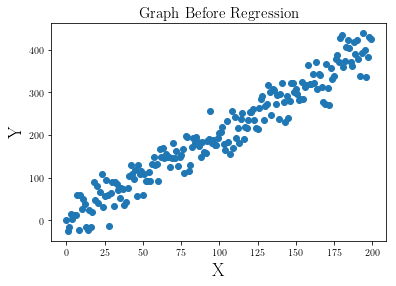
\includegraphics[scale = 0.6]{Line.png}
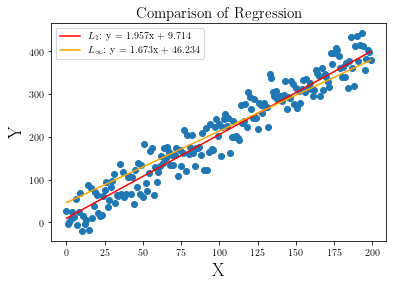
\includegraphics[scale = 0.6]{Comparison.png}
\caption{Using different types of regression produces entirely different regression lines. In general, after running the regression multiple times, $L_1$ regression was generally found to produce a line of greater slope that $L_\infty$. As a result, the intercept of the $L_\infty$ regression was usually higher than the intercept of $L_1$ regression.}
\end{figure*}
In this section, we use CVXPY to perform both $L_1$ and $L_\infty$ regression on a given dataset. The code used to generate the data, as well as the plots are available \href{https://github.com/thetruejacob/CS166/blob/master/Network%20Simulation%20Assignment/Network%20Simulation.ipynb}{here}.






\end{document}